Entrambi i protocolli sono stati sviluppati al livello applicativo sopra lo stack \verb+TCP/IP+.
Viene garantita la confidenzialità della comunicazione evitando intercettazioni o manomissioni dei messaggi tramite il protocollo \verb+TLS+ attraverso il layer del trasporto \verb+TCP+, risultando trasparente per gli strati superiori \cite{Rfc5246}.

I dati necessari per instaurare questa comunicazione protetta (\textit{handshake}) vengono negoziati prima che il primo byte dell'applicativo venga inviato.
La volontà di cifrare questi dati deve essere necessariamente specificata all'inizio della connessione, per permettere lo scambio delle chiavi necessarie a garantire la giusta riservatezza, comportando un leggero sovraccarico (\textit{overhead}) computazionale per tutta la durata della comunicazione.

Cifrando i dati dell'applicativo con le chiavi scambiate inizialmente tra i due interlocutori (\textit{Alice} e \textit{Bob}), un terzo personaggio (\textit{Charlie}), difficilmente riuscirebbe a comprendere questa comunicazione.

\begin{figure}[H]
  \centering
  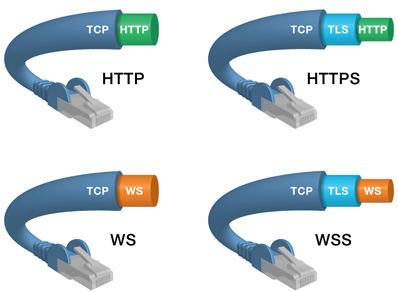
\includegraphics[scale=0.8, keepaspectratio]{tls}
  \caption{Astrazione della connessione tramite TLS attraverso il protocollo TCP}
  \label{fig:tls}
\end{figure}

Le porte di default del \textit{server} per accettare questo tipo di connessioni differiscono rispetto a quelle prive di cifratura e sono:
\begin{table}[H]
  \begin{center}
  \begin{tabular}{| l | l | c |}
    \hline
    Protocollo & Porta & Sicuro \\ \hline
    \verb+HTTP+ & \textbf{80} & \ding{55} \\
    \verb+HTTPS+ & \textbf{443} & \ding{51} \\ \hline
    \verb+WS+ & \textbf{80} & \ding{55} \\
    \verb+WSS+ & \textbf{443} & \ding{51} \\ \hline
    \verb+MQTT+ & \textbf{1883} & \ding{55} \\
    \verb+MQTTS+ & \textbf{8883} & \ding{51} \\ \hline
  \end{tabular}
  \label{tab:securityPorts}
  \caption{Elenco dei protocolli con le loro porte e relativa cifratura}
  \end{center}
\end{table}
